%\documentclass[10pt,handout]{beamer}
\documentclass[11pt]{beamer}\usepackage[]{graphicx}\usepackage[]{color}
%% maxwidth is the original width if it is less than linewidth
%% otherwise use linewidth (to make sure the graphics do not exceed the margin)
\makeatletter
\def\maxwidth{ %
  \ifdim\Gin@nat@width>\linewidth
    \linewidth
  \else
    \Gin@nat@width
  \fi
}
\makeatother

\definecolor{fgcolor}{rgb}{0.196, 0.196, 0.196}
\newcommand{\hlnum}[1]{\textcolor[rgb]{0.063,0.58,0.627}{#1}}%
\newcommand{\hlstr}[1]{\textcolor[rgb]{0.063,0.58,0.627}{#1}}%
\newcommand{\hlcom}[1]{\textcolor[rgb]{0.588,0.588,0.588}{#1}}%
\newcommand{\hlopt}[1]{\textcolor[rgb]{0.196,0.196,0.196}{#1}}%
\newcommand{\hlstd}[1]{\textcolor[rgb]{0.196,0.196,0.196}{#1}}%
\newcommand{\hlkwa}[1]{\textcolor[rgb]{0.231,0.416,0.784}{#1}}%
\newcommand{\hlkwb}[1]{\textcolor[rgb]{0.627,0,0.314}{#1}}%
\newcommand{\hlkwc}[1]{\textcolor[rgb]{0,0.631,0.314}{#1}}%
\newcommand{\hlkwd}[1]{\textcolor[rgb]{0.78,0.227,0.412}{#1}}%

\usepackage{framed}
\makeatletter
\newenvironment{kframe}{%
 \def\at@end@of@kframe{}%
 \ifinner\ifhmode%
  \def\at@end@of@kframe{\end{minipage}}%
  \begin{minipage}{\columnwidth}%
 \fi\fi%
 \def\FrameCommand##1{\hskip\@totalleftmargin \hskip-\fboxsep
 \colorbox{shadecolor}{##1}\hskip-\fboxsep
     % There is no \\@totalrightmargin, so:
     \hskip-\linewidth \hskip-\@totalleftmargin \hskip\columnwidth}%
 \MakeFramed {\advance\hsize-\width
   \@totalleftmargin\z@ \linewidth\hsize
   \@setminipage}}%
 {\par\unskip\endMakeFramed%
 \at@end@of@kframe}
\makeatother

\definecolor{shadecolor}{rgb}{.97, .97, .97}
\definecolor{messagecolor}{rgb}{0, 0, 0}
\definecolor{warningcolor}{rgb}{1, 0, 1}
\definecolor{errorcolor}{rgb}{1, 0, 0}
\newenvironment{knitrout}{}{} % an empty environment to be redefined in TeX

\usepackage{alltt}
%\documentclass[11pt, handout]{beamer}
%\usepackage{handoutWithNotes}
%\usepackage{pgfpages}
\usepackage{etex} % helps fix \newdimen error which is cause when ctable is loaded with other packages
\usepackage{comment}
\usepackage{ctable}
\usepackage{amsmath,amsthm,amssymb}
\usepackage{url}
\usepackage{color, colortbl}
\usepackage{tikz}
\usetikzlibrary{shapes.geometric, arrows,shapes.symbols,decorations.pathreplacing}
\tikzstyle{startstop} = [rectangle, rounded corners, minimum width=3cm, minimum height=1cm,text centered, draw=black, fill=red!30,text width=2.0cm]
\tikzstyle{io} = [trapezium, trapezium left angle=70, trapezium right angle=110, minimum width=2cm, minimum height=1cm, text centered, draw=black, fill=blue!30,text width=1.5cm]
\tikzstyle{process} = [rectangle, minimum width=1cm, minimum height=1cm, text centered, draw=black, fill=orange!30,text width=2cm]
\tikzstyle{decision} = [diamond, minimum width=2cm, minimum height=1cm, text centered, draw=black, fill=green!30]
\tikzstyle{arrow} = [thick,->,>=stealth]
\tikzstyle{both} = [thick,<->,>=stealth, red]

\tikzset{myshade/.style={minimum size=.4cm,shading=radial,inner color=white,outer color={#1!90!gray}}}
\newcommand\mycirc[1][]{\tikz\node[circle,myshade=#1]{};}
\newcommand\myrect[1][]{\tikz\node[rectangle,myshade=#1]{};}
\newcommand\mystar[1][]{\tikz\node[star,star points=15,star point height=2pt,myshade=#1]{};}
\newcommand\mydiamond[1][]{\tikz\node[diamond,myshade=#1]{};}
\newcommand\myellipse[1][]{\tikz\node[ellipse,myshade=#1]{};}
\newcommand\mykite[1][]{\tikz\node[kite,myshade=#1]{};}
\newcommand\mydart[1][]{\tikz\node[dart,myshade=#1]{};}
\newcommand\mycloud[1][]{\tikz\node[cloud,myshade=#1]{};}

%\usepackage{subcaption}
\usepackage{subfig}
%\usepackage{caption}

\mode<presentation>
\usetheme{Hannover}
\usecolortheme{rose}
\setbeamertemplate{navigation symbols}{}
\setbeamertemplate{footline}[frame number]
\setbeamertemplate{caption}[numbered]
\setbeamertemplate{frametitle}[default][left]

\usepackage[]{hyperref}
\hypersetup{
    unicode=false,          
    pdftoolbar=true,        
    pdfmenubar=true,        
    pdffitwindow=false,     % window fit to page when opened
    pdfstartview={FitH},    % fits the width of the page to the window
    pdftitle={atelier R GERAD},    % title
    pdfauthor={Sahir Rai Bhatnagar},     % author
    pdfsubject={Subject},   % subject of the document
    pdfcreator={Sahir Rai Bhatnagar},   % creator of the document
    pdfproducer={Sahir Rai Bhatnagar}, % producer of the document
    pdfkeywords={}, % list of keywords
    pdfnewwindow=true,      % links in new window
    colorlinks=true,       % false: boxed links; true: colored links
    linkcolor=red,          % color of internal links (change box color with linkbordercolor)
    citecolor=blue,        % color of links to bibliography
    filecolor=black,      % color of file links
    urlcolor=cyan           % color of external links
}

\RequirePackage{color}

% define a bunch of colors
\definecolor{gray}{RGB}{110,110,110}
\definecolor{darkgray}{RGB}{100,100,100}
\definecolor{lightgray}{RGB}{200,200,200}
\definecolor{turquoise}{RGB}{81,193,188}
\definecolor{tomato}{RGB}{229,136,136}
\definecolor{mandarina}{RGB}{229,169,25}
\definecolor{foreground}{RGB}{81,141,193}
\definecolor{background}{RGB}{246,244,240}
\definecolor{highlight}{RGB}{229,169,25}
\definecolor{lowlight}{RGB}{200,200,200}

% some convenient commands
\newcommand{\code}[1]{\texttt{#1}}
\newcommand{\high}[1]{\textcolor{highlight}{#1}}
\newcommand{\low}[1]{\textcolor{lowlight}{#1}}
\newcommand{\highcode}[1]{\textcolor{highlight}{\texttt{#1}}}

%\setbeamercolor{subtitle}{fg=turquoise}

%\pgfpagesuselayout{4 on 1}[a4paper, landscape, border shrink=5mm]
%\pgfpagesuselayout{2 on 1 with notes landscape}[a4paper, border shrink=5mm]
\IfFileExists{upquote.sty}{\usepackage{upquote}}{}
\begin{document}





\title[Atelier sur le logiciel R]{Atelier sur le logiciel R}
\subtitle{Un introduction \`{a} la programmation en R}

\author[]{Sahir Rai Bhatnagar%
\thanks{\href{https://github.com/sahirbhatnagar/atelier-R-GERAD}{https://github.com/sahirbhatnagar/atelier-R-GERAD}%
}}

\date{29 juillet 2015}

%\makebeamertitle

\maketitle

\begin{frame}{Remerciements}
% \hspace*{-1.9cm}\parbox[t]{\textwidth}
%\frametitle{Acknowledgements}
\begin{columns}[c] % The "c" option specifies centered vertical alignment while the "t" option is used for top vertical alignment

\column{.45\textwidth} % Left column and width

\begin{itemize}
%\scriptsize
\item Dr. Vahid Partovi Nia
\item Greg Voisin
\item Ross Ihaka et Robert Gentleman
\item Toi
\end{itemize}

\column{.45\textwidth} % Right column and width
\begin{figure}

\includegraphics[width=0.6\columnwidth]{gerad.png}\\[2mm]

\includegraphics[width=0.6\columnwidth]{udem.png}\\[5mm]

\includegraphics[width=0.6\columnwidth]{hec.png}
%\includegraphics[width=0.7\columnwidth]{Logo-LUDMER.jpg}
\end{figure}

\end{columns}
\end{frame}


\begin{frame}{Avis \#1}
\begin{itemize}
\item N'h\'{e}sitez pas \`{a} posez des questions
\end{itemize}
\end{frame}

\begin{frame}{Avis \#2}
\begin{figure}

\includegraphics[width=1.0\columnwidth]{rstudio.png}\\[5mm]

\includegraphics[width=0.2\columnwidth]{rlogo.png}\\[5mm]
%\includegraphics[width=0.2\columnwidth]{LaTeX_logo.png}
\end{figure}

\textit{Je ne travaille pas pour, ni un auteur de ces logiciels.}

\end{frame}

\begin{frame}{Avis \#3}

\begin{itemize}
\item Le mat\'{e}riel pour cet atelier est bas\'{e} sur plusieurs resources
\item Voir ce lien pour une liste compl\`{e}te de r\'{e}f\'{e}rences: \href{https://github.com/sahirbhatnagar/atelier-R-GERAD}{https://github.com/sahirbhatnagar/atelier-R-GERAD}
\item Je vous sugg\`{e}re le livre par Vincent Goulet
\end{itemize}


\begin{figure}

\includegraphics[width=0.4\columnwidth]{goulet.png}
\end{figure}


\end{frame}


\begin{frame}[plain]{C'est parti}
\hspace*{-1.5cm}\parbox[t]{\textwidth}{
\begin{center}
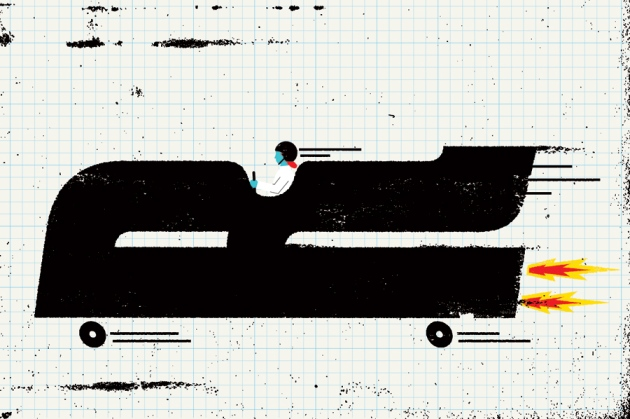
\includegraphics[scale=0.51]{introR.jpg}
\end{center}
}
\end{frame}



\section{1. Pr\'{e}sentation du langage R}

\setbeamercolor{normal text}{fg=gray,bg=black}
\begin{frame}[plain]
\hspace*{-1.0cm}\parbox[t]{\textwidth}{
 \begin{center}
  \Huge{\textcolor{white}{1. Pr\'{e}sentation du langage R}}
 \end{center}
 }
\end{frame}

\setbeamercolor{normal text}{fg=gray,bg=white}
\subsection{Pourquoi vous \^{e}tes l\`{a}?}

\begin{frame}
 \begin{center}
  \Huge{\textcolor{red}{Pourquoi vous \^{e}tes l\`{a}?}}
 \end{center}
\end{frame}


\begin{frame}{Le langage R gagne en popularit\'{e}}

\vspace{0.1in}

\begin{center}
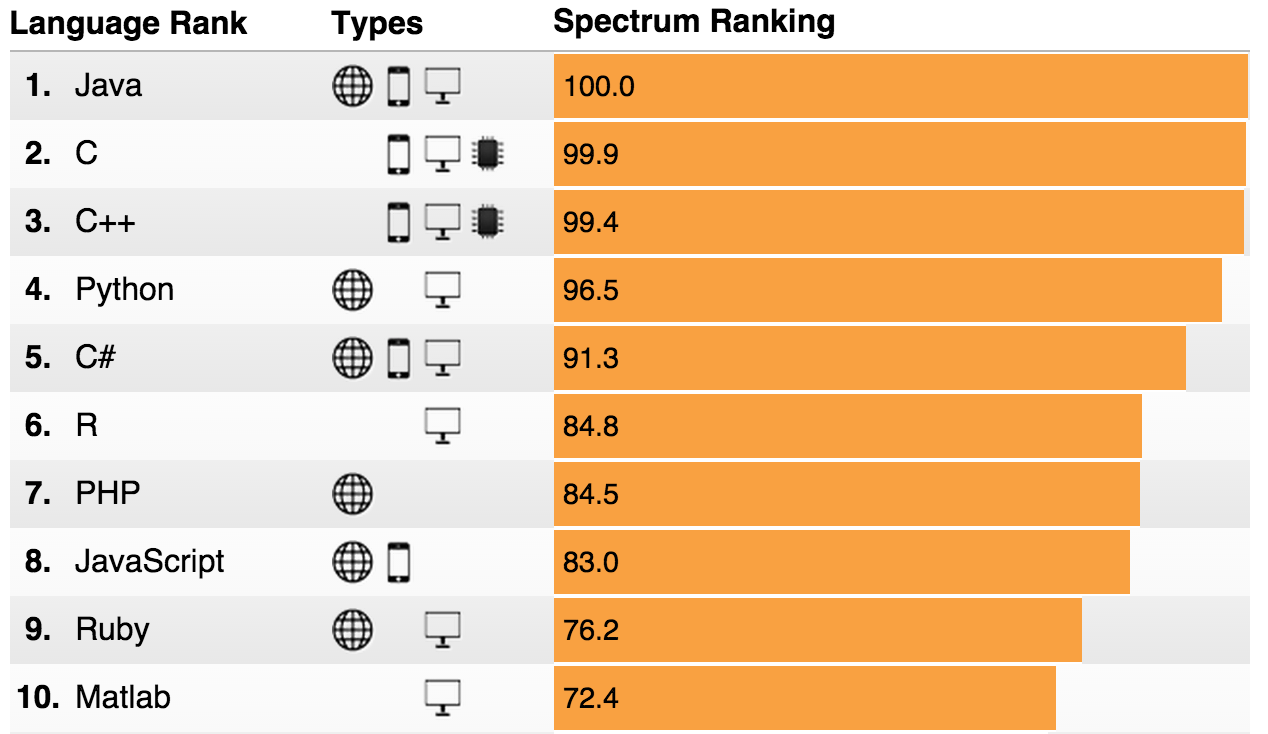
\includegraphics[scale=0.40]{rankings.png}
\end{center}

\vspace{0.2in}

Les meilleurs langage de programmation en 2015 selon \href{http://spectrum.ieee.org/computing/software/the-2015-top-ten-programming-languages}{\mbox{IEEE Spectrum}} \\
\end{frame}


\begin{frame}{Plus de 100,000 questions pos\'{e}s dans les forums}


\includegraphics[scale=0.40]{stack.png}
\newline
\vspace{0.1in}
%\footenotesize{source: http://r4stats.com/articles/popularity/}
\end{frame}




\begin{frame}{Nombres d'emplois}

\begin{center}
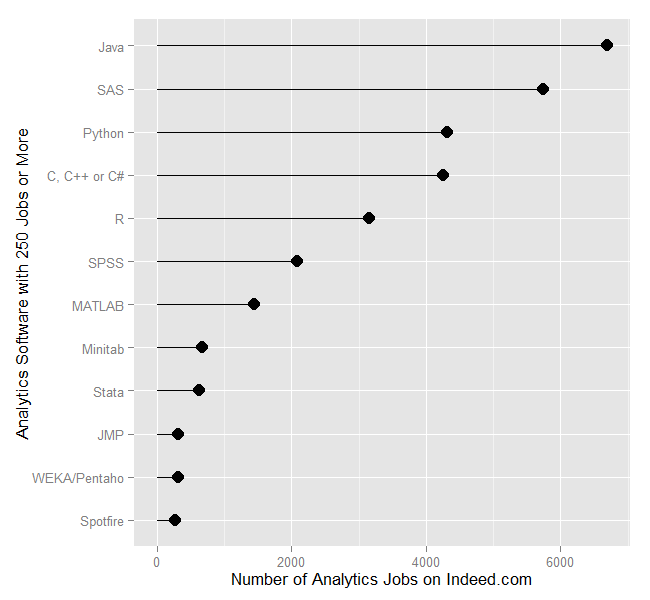
\includegraphics[scale=0.47]{jobs.png}
\end{center}

\vspace{0.05in}

r\'{e}f\'{e}rence: \href{http://r4stats.com/articles/popularity/}{http://r4stats.com/articles/popularity/}\\

\end{frame}



\begin{frame}{Utilis\'{e} dans plusieurs domaines}

\begin{center}
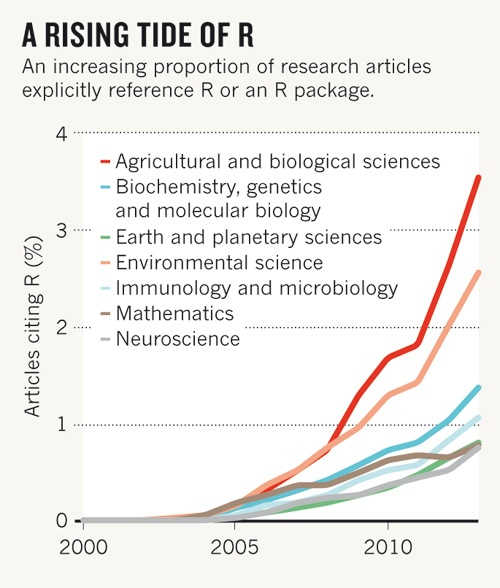
\includegraphics[scale=0.31]{citeR.jpg}
\end{center}

\vspace{0.05in}

Publi\'{e} dans \href{http://www.nature.com/news/programming-tools-adventures-with-r-1.16609}{\textit{Nature}}
\end{frame}



\subsection{Bref historique}

\begin{frame}
 \begin{center}
  \Huge{\textcolor{red}{Bref historique}}
 \end{center}
\end{frame}


\begin{frame}{\`{A} l'origine de R fut le S par John M. Chambers}
\begin{center}
\begin{figure}
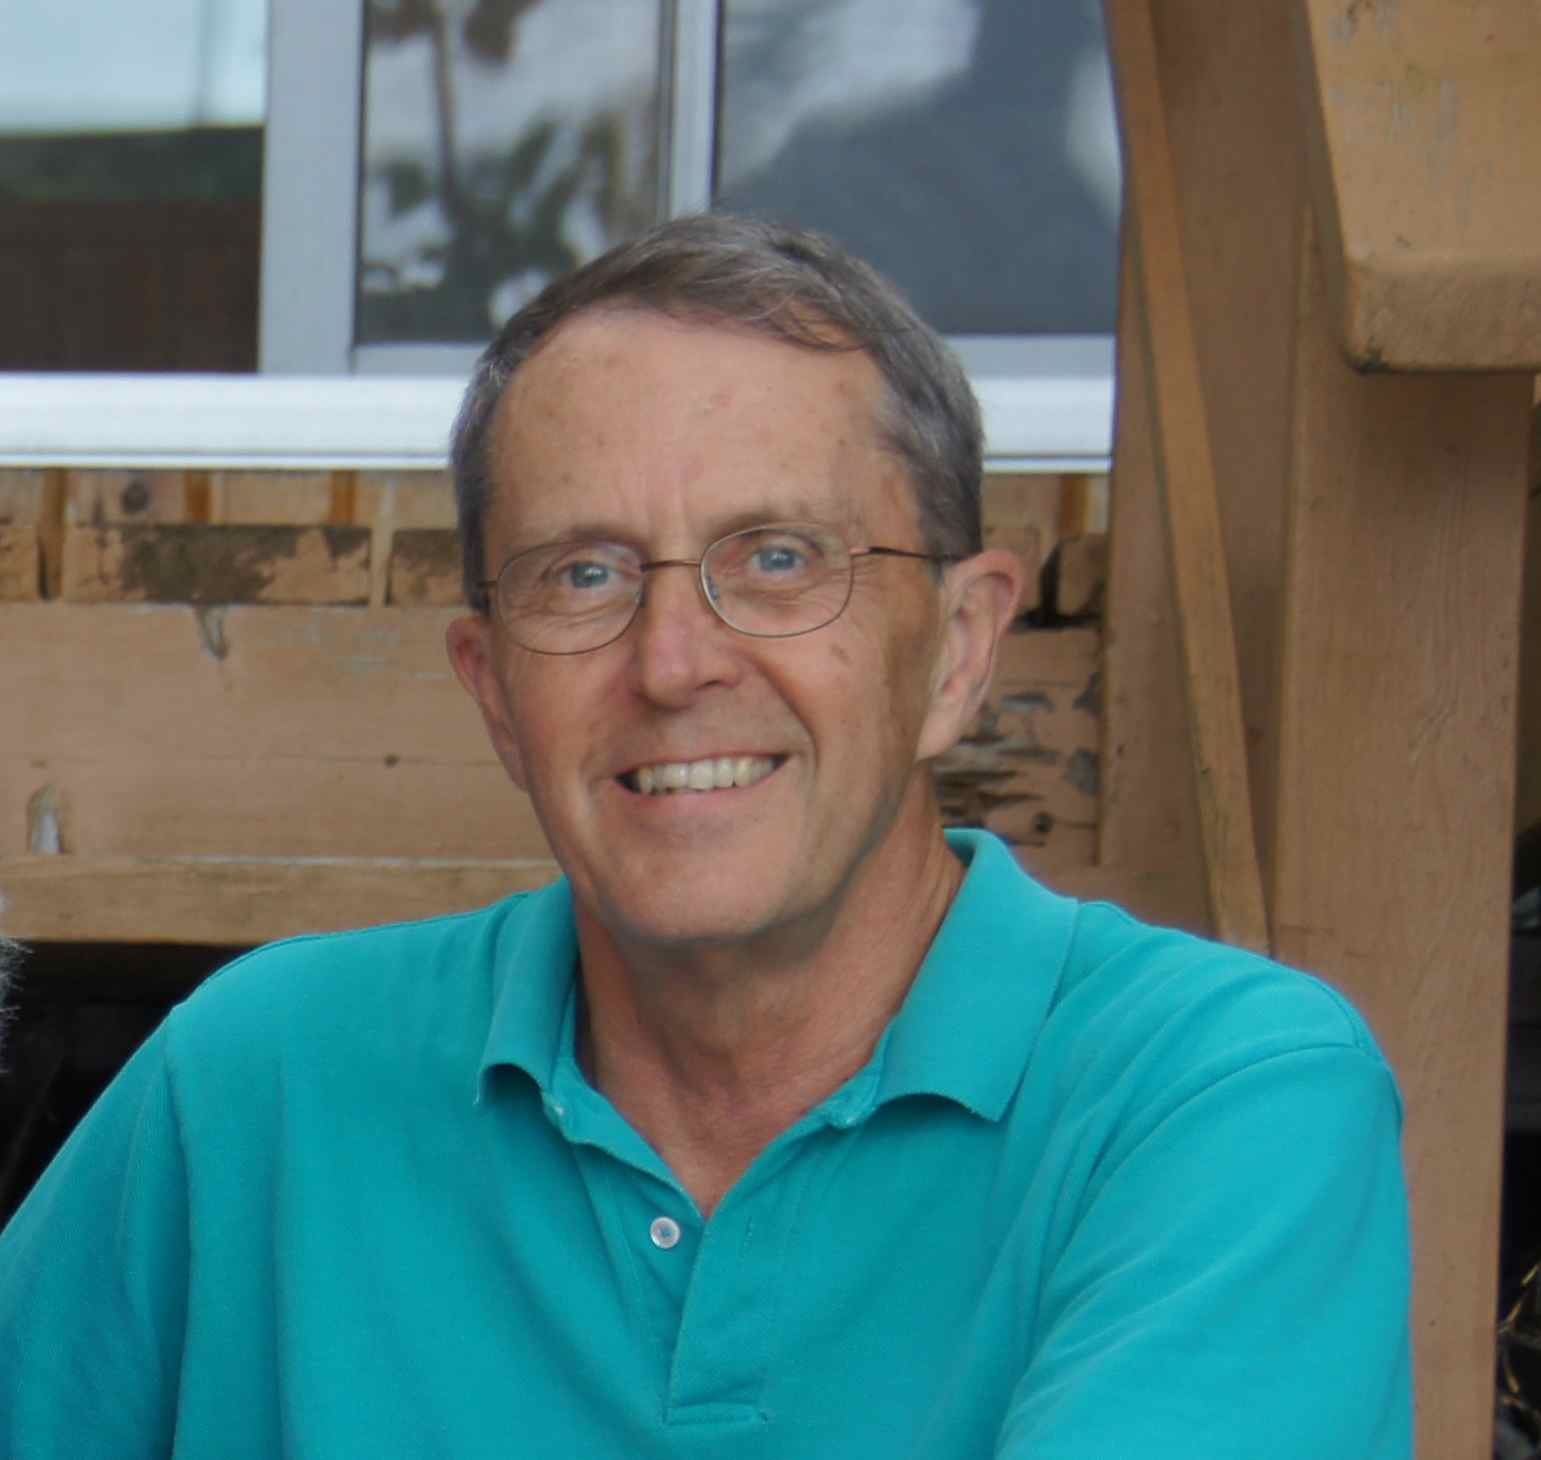
\includegraphics[scale=0.10]{john.jpg}
\caption{S, un langage pour programmmer avec des donn\'{e}es, developp\'{e} chez Bell Laboratories dans les ann\'{e}es 1970 par une \'{e}quipe de chercheurs men\'{e}e par John M. Chambers}
\end{figure}
\end{center}
\end{frame}


\begin{frame}{Cr\'{e}ateurs}
\begin{center}
\begin{figure}
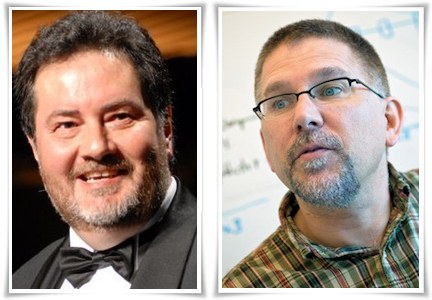
\includegraphics[scale=0.60]{rr.jpg}
\caption{Inspir\'{e}s par le S, Ross Ihaka (gauche) et Robert Gentleman de l'Universit\'{e} d'Auckland en Nouvelle-Z\'{e}lande ont lanc\'{e} la premi\`{e}re version de R en 1996}
\end{figure}
\end{center}
\end{frame}


\begin{frame}{Logiciel Libre}
\begin{itemize}
  \setlength\itemsep{2em}
\item 1990-2010: le S a principalement \'{e}t\'{e} popularis\'{e} par une mise en oeuvre commerciale nomm\'{e}e S-PLUS
\pause \item Fin des ann\'{e}es 2000: L'utilisation de S-PLUS diminue en faveur du R, surtout dans les milieux acad\'{e}miques
\pause \item 2 raisons qui ont fortement contribu\'{e} \`{a} la perte d'influence de S-PLUS
\begin{enumerate}
\item \normalsize Disponible gratuitement
\pause \item Ouvert aux contribution de tous
\end{enumerate}
\end{itemize}
\end{frame}



\subsection{Charact\'{e}ristiques de R}

\begin{frame}
 \begin{center}
  \Huge{\textcolor{red}{Charact\'{e}ristiques de R}}
 \end{center}
\end{frame}



\begin{frame}{Langage de programmation interpr\'{e}t\'{e}}
\begin{itemize}
  \setlength\itemsep{2em}
\item Langage de programmation interpr\'{e}t\'{e}
\pause \item Oppos\'{e} d'un langage compil\'{e}s (\code{C} ou le \code{C++})
\pause \item Le programme qu'on lance pour utiliser R est l'interpr\`{e}te
\pause \item Celui-ci prend des commandes dans le langage R, qu'il ex\`{e}cutera imm\'{e}diatement
\pause \item  Autre exemple: \code{Excel}
\end{itemize}
\end{frame}


\begin{frame}{Logiciel libre (\textit{Open Source})}

\begin{itemize}
  \setlength\itemsep{2em}
\item D\'{e}veloppement actif pour la cr\'{e}ation de nouveau outils dans plusieurs domaines $\rightarrow$ \href{https://cran.r-project.org/web/views/}{https://cran.r-project.org/web/views/} 
\item Facilement voir le code des autres avec GitHub $\rightarrow$ \href{http://www.r-pkg.org/}{http://www.r-pkg.org/}
\end{itemize}

%\begin{center}
%\begin{figure}
%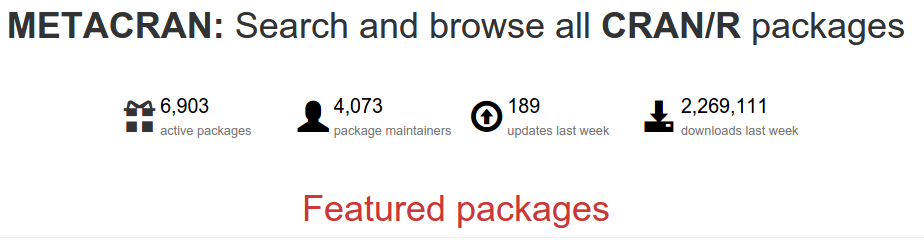
\includegraphics[scale=0.35]{meta.png}
%\caption{\href{http://www.r-pkg.org/}{http://www.r-pkg.org/}}
%\end{figure}
%\end{center}

\end{frame}






\begin{frame}{O\`{u} trouver de la documentation}
\begin{itemize}
\item \texttt{help.start()} for general help
\item \texttt{help(function\_name)} or \texttt{?function\_name}
\item \texttt{??search\_term}
\item \texttt{example(function\_name)}
\item  \href{http://stackoverflow.com/questions/tagged/r}{\underline{\textcolor{blue}{Stackoverflow}}}
\item refer to 'Short intro to R' document posted on MyCourses
\item Google it
\end{itemize}
\end{frame}


\begin{frame}{Clavier Mac}

\vspace{0.1in}

\begin{center}
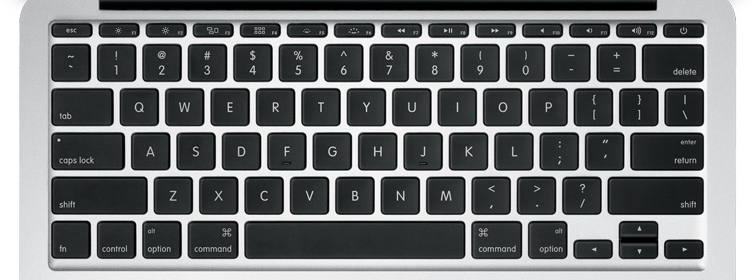
\includegraphics[scale=0.40]{mackey.jpg}
\end{center}

\end{frame}



\begin{frame}{Clavier PC}

\vspace{0.1in}

\begin{center}
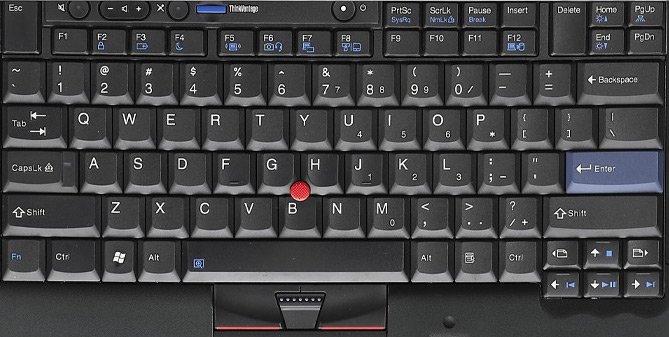
\includegraphics[scale=0.40]{pckey.jpg}
\end{center}

\end{frame}



%\subsection{Bref Historique et description}





\subsection{D\'{e}marrer une session}

\begin{frame}
 \begin{center}
  \Huge{\textcolor{red}{D\'{e}marrer une session}}
 \end{center}
\end{frame}











\section{2. Bases du langage R}

\setbeamercolor{normal text}{fg=gray,bg=black}
\begin{frame}[plain]
\hspace*{-1.0cm}\parbox[t]{\textwidth}{
 \begin{center}
  \Huge{\textcolor{white}{2. Bases du langage R}}
 \end{center}
 }
\end{frame}

\setbeamercolor{normal text}{fg=gray,bg=white}
\subsection{Les objets R}

\begin{frame}
 \begin{center}
  \Huge{\textcolor{red}{Les objets R}}
 \end{center}
\end{frame}





\section{3. Graphiques}

\setbeamercolor{normal text}{fg=gray,bg=black}
\begin{frame}[plain]
\hspace*{-1.0cm}\parbox[t]{\textwidth}{
 \begin{center}
  \Huge{\textcolor{white}{3. Graphiques}}
 \end{center}
 }
\end{frame}

\setbeamercolor{normal text}{fg=gray,bg=white}
\subsection{Les objets R}

\begin{frame}
 \begin{center}
  \Huge{\textcolor{red}{Les objets R}}
 \end{center}
\end{frame}




\section{4. Statistiques}

\setbeamercolor{normal text}{fg=gray,bg=black}
\begin{frame}[plain]
\hspace*{-1.0cm}\parbox[t]{\textwidth}{
 \begin{center}
  \Huge{\textcolor{white}{4. Statistiques}}
 \end{center}
 }
\end{frame}

\setbeamercolor{normal text}{fg=gray,bg=white}
\subsection{Les objets R}

\begin{frame}
 \begin{center}
  \Huge{\textcolor{red}{Les objets R}}
 \end{center}
\end{frame}



\section{5. Cr\'{e}er des rapports reproductibles}

\setbeamercolor{normal text}{fg=gray,bg=black}
\begin{frame}[plain]
\hspace*{-1.0cm}\parbox[t]{\textwidth}{
 \begin{center}
  \Huge{\textcolor{white}{5. Cr\'{e}er des rapports}}
 \end{center}
 }
\end{frame}

\setbeamercolor{normal text}{fg=gray,bg=white}
\subsection{Les objets R}

\begin{frame}
 \begin{center}
  \Huge{\textcolor{red}{Les objets R}}
 \end{center}
\end{frame}
















\end{document}
